The results here are from a single run of our program on each generator, using Dieharder's standard test suite produced by the \texttt{-a} flag. These tests may leave the user reasonably satisfied with the results, but it is very possible that a test failure may mean nothing at all. These failures may simply be due to chance, a poor seed, or not enough testing. A more robust version of these tests is available in Dieharder, but running these tests on a single generator can take in excess of 24 hours. Unfortunately, we were not able to run the more robust versions of these tests, or average out several 1 hour runs, as would be ideal. Additionally due to the predictably low speed of the RANLUX generator, we are forced to present only partial test results for RANLUX. As RANLUX was two orders of magnitude slower than other RNGs implemented, it would have taken two orders of magnitude longer to allow the test to complete.

Overall, the RNGs that we implemented performed as expected. Namely, they performed similarly to what literature, as well as similar (if not identical) implementations in the GNU Scientific Library produced. All RNGs (with the notable and expected exception of RANDU) passed the majority of the tests, with at only a few failure, and a few weak results which could very possibly pass if tested with different seeds. Statistics for passes, weaks, and failures are presented in visual form in Figure~\ref{fig:passesweaksfails} and tabularly in Table~\ref{tab:passesweaksfails}.

\begin{figure}[tb]
    \begin{center}
        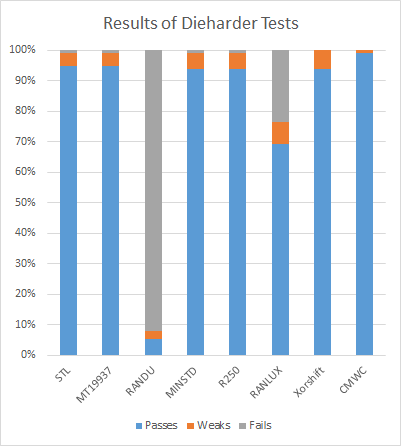
\includegraphics[width=\linewidth]{figures/passesweaksfails.png}
    \end{center}
    \caption{Percentage bar graph of results of Dieharder test results for implemented RNGS.}
    \label{fig:passesweaksfails}
\end{figure}

% http://www.tablesgenerator.com/
\begin{table}[tb]
    \caption{Table displaying Dieharder results for the implemented RNGs.}
    \label{tab:speed}
    \begin{center}
        \begin{tabular}{l|ccc}
        \hline
        \hline
\textbf{RNG Name} & \textbf{Passes} & \textbf{Weaks} & \textbf{Fails} \\
        \hline
STL               & 108             & 5              & 1              \\
MT19937           & 108             & 5              & 1              \\
RANDU             & 6               & 3              & 105            \\
MINSTD            & 107             & 6              & 1              \\
R250              & 107             & 6              & 1              \\
RANLUX            & 79              & 8              & 27             \\
Xorshift          & 107             & 7              & 0              \\
CMWC              & 113             & 1              & 0 \\
        \hline
        \hline
        \end{tabular}
    \end{center}
\end{table}


Another metric worth measuring is RNG speed. This metric has been alluded in Section~\ref{sec:classes}, but is formally measured in random numbers per second. Luckily, Dieharder measures this metric already. As expected, the STL implementation of the Mersenne Twister is quite fast (as is much of the STL), and the RANLUX implementation is slow (because it must discard so many numbers to keep the quality of output high). Of the other RNGs, our Mersenne Twister is the most complicated, and as a result it is the slowest. RANDU is simple and fast, and the other algorithms hover around the same speed. The data is presented graphically in Figure~\ref{fig:speed} and tabularly in Table~\ref{tab:speed}. These speeds were measured on a laptop with an Intel Core i7-4600U CPU @ 2.10GHz with 4 cores.

It is important to remember that these speeds must be considered to be relative. These RNGs must be piped through the shell, as opposed to the GNU Scientific Library RNGs built into the Dieharder binary, and as a result, they can be passed to Dieharder faster.

\begin{figure}[tb]
    \begin{center}
        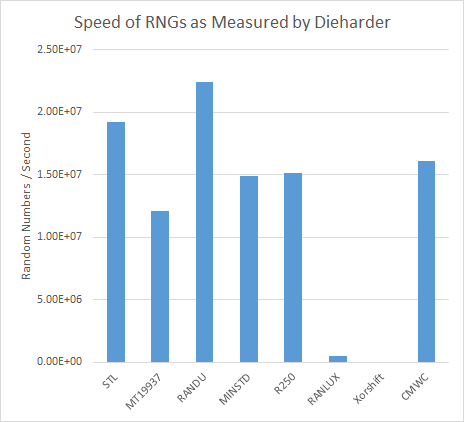
\includegraphics[width=\linewidth]{figures/speed.png}
    \end{center}
    \caption{Speed of implemented RNGs in random numbers per second as measured by Dieharder.}
    \label{fig:speed}
\end{figure}

% http://www.tablesgenerator.com/
\begin{table}[tb]
    \caption{Table displaying speeds of implemented RNGs as measured by Dieharder.}
    \label{tab:passesweaksfails}
    \begin{center}
        \begin{tabular}{l|c}
        \hline
        \hline
\textbf{RNG Name} & \textbf{Speed} \\
        \hline
STL       &  1.91E+07  \\
MT19937   &  1.26E+07  \\
RANDU     &  2.18E+07  \\
MINSTD    &  1.49E+07  \\
R250      &  1.51E+07  \\
RANLUX    &  5.00E+05  \\
Xorshift  &  7.90E+06  \\
CMWC      &  4.30E+06  \\
TinyMT    &  7.97E+06  \\

        \hline
        \hline
        \end{tabular}
    \end{center}
\end{table}


Finally, a measure that cannot be easily determined empirically, and instead falls under analytical testing, is that of period length. As described in Section~\ref{sec:classes}, as the complexity of the generator goes up, the period also goes up. The Mersenne Twister has a particularly large period several orders of magnitude larger than more simple ones, expect for the particular CMWC generator chosen. Though this generator stores far more state than the standard Mersenne Twister implementation, it is significantly faster and has a period several orders of magnitude greater than the other generators. Period lengths for implemented RNGS are displayed tabularly in Table~\ref{tab:period}.

% http://www.tablesgenerator.com/
\begin{table}[tb]
    \caption{Table of periods of implemented RNGs.}
    \label{tab:period}
    \begin{center}
        \begin{tabular}{l|c}
        \hline
        \hline
\textbf{RNG Name} & \textbf{Period Length} \\
        \hline
STL               & $2^{19937}-1$  \\
MT19937           & $2^{19937}-1$  \\
RANDU             & $2^{29}$       \\
MINSTD            & $2^{31}-1$     \\
R250              & $2^{250}-1$    \\
RANLUX            & $10^{171}$       \\
Xorshift          & $2^{128}-1$    \\
CMWC              & $2^{131104}$   \\
TinyMT            & $2^{127}-1$    \\
        \hline
        \hline
        \end{tabular}
    \end{center}
\end{table}

